\chapter{Metodologia}
\label{capitolometodologia}
In questo capitolo sono descritti nel dettaglio gli algoritmi, le strutture, le librerie ed il linguaggio utilizzato per la collezione, la manipolazione dei dati di Crunchbase\footnote{Crunchbase: \url{https://www.crunchbase.com/}.}. Infine, viene descritto l'approccio alla validazione dei dati Crunchbase che vengono confrontati con i dati presenti nel MIMI.\par
\setminted{fontsize=\footnotesize,baselinestretch=0.9,fontfamily = courier}
\begin{figure}[t]
    \centering
    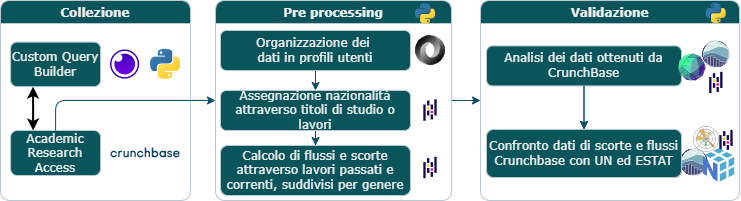
\includegraphics[width=1\textwidth]{images/SVG/diagram2.png}
    \caption{Diagramma della metodologia}
    \label{fig:digram}
\end{figure}

Come mostrato in Figura \ref{fig:digram}, la metodologia proposta è divisa in tre fasi: collezione, pre-processing e validazione dei dati. 
La collezione dei dati è stata effettuata attraverso due diversi metodi: 
\begin{itemize}
    \item Custom Query Builder
    \item Crunchbase Academic Research Access
\end{itemize}
Il Custom Query Builder è stato utilizzato per la raccolta dei dati fino a che non è stata ottenuta la possibilità di accedere ai dati tramite Academic Research Access. 
I dati collezionati da Crunchbase seguendo l'approccio descritto in Sezione \ref{academic_access_section}, sono preprocessati al fine di estrapolare le informazioni relative agli utenti, ai flussi e alle scorte migratorie. 
Dopo la collezione e il preprocessing, è stata affrontata la validazione dei dati. Con questo obiettivo, le scorte ed i flussi calcolati a partire dai dati collezionati da Crunchbase sono stati confrontati con quelli nel MIMI mediante un analisi di correlazione.
Inoltre, i risultati sono stati visualizzati mediante 
\textit{chord diagram}\footnote{Il chord diagram, in italiano, diagramma a corda rappresenta i flussi e le connessioni tra diverse entità, chiamate nodi. Ciascuna entità è rappresentata da un segmento del perimetro circolare. Gli archi sono tracciati tra entità connesse. Inoltre, la dimensione dell'arco è proporzionale all'importanza o dimensione dell'entità misurata (scorte o flussi) \footnote{(From Data to Viz: Chord Diagram \url{https://www.data-to-viz.com/graph/chord.html}.}}, seguendo diversi livelli di aggregazione geografica.

\section{Collezione dei dati}
\label{sezionecollezionedati}
La collezione dei dati è avvenuta attraverso due metodi: il Custom Query Builder e l'Academic Research Access. Il Custom Query Builder è stato realizzato mediante lo studio del meccanismo di \textit{query} offerto dalla piattaforma Crunchbase. In un secondo momento è stato ottenuto l'accesso accademico ai dati che ha permesso di prelevare i dati ufficiali da Crunchbase.

Per determinare la validità dei dati ottenuti si confrontano con i dati del MIMI dataset, per scorte e flussi. Ogni confronto con i dati ufficiali consiste nel calcolo della correlazione e la visualizzazione dei dati su grafici di dispersione. 

\subsection{Query Builder}
\label{sottosezionequerybuilder}
Per ottenere i dati si è scelto, nella fase iniziale, di sfruttare il Query Builder offerto dalla piattaforma Crunchbase.
Il Query Builder permette di filtrare in base alle entità, tra cui persone, compagnie, investitori, acquisizioni.
Dato che l'obiettivo di questa tesi è studiare la migrazione delle persone altamente specializzate abbiamo limitato la collezione dei dati alle persone.
Il Query Builder permette di filtrare ulteriormente la ricerca sulla base di varie informazioni degli utenti, tra cui la carriera lavorativa, i titoli di studio, eventi ai quali hanno partecipato e il genere.

Una volta eseguita una ricerca tramite il Query Builder, il sito pubblico di Crunchbase  restituisce i primi 5 profili che soddisfano la query più il numero totale di profili. Il nostro approccio non utilizza i profili individuali, ma salva solamente il numero totale di profili, che saranno interpretati come la dimensione delle scorte e flussi migratori. Questo approccio rispetta la privacy degli utenti e risulta in numeri aggregati e anonimizzati. 


Per studiare la migrazione abbiamo costruito dei query che selezionano i soli profili utenti di persone che hanno conseguito la laurea in un set di paesi selezionati\footnote{Stati Uniti, Canada, India, Filippine, Pakistan, Australia, Cina, Singapore, Brasile, Giappone e continente europeo.} (lo stato di laurea sarà considerato un proxy per la nazionalità). Per ottenere le scorte annuali è stato estratto il numero di persone che lavoravano il 1° Gennaio di ogni anno, dal 2010 al 2020, in ciascuno degli stati selezionati. 
Infine, per ottenere i flussi, è stato estratto il numero di persone che hanno cambiato impiego durante ciascun anno, dal 2010 al 2020, sposandosi tra gli stati selezionati. 


Al fine di automatizzare il processo di collezione abbiamo deciso di applicare tecniche di \textit{reverse engineering}\footnote{Ingegneria/ingegnerizzazione inversa.}. 
Grazie alla comprensione del meccanismo di comunicazione del sito è stato realizzato il Custom Query Builder (Sezione \ref{customquerybuilder}), che genera automaticamente le richieste da inviare, le invia e ne gestisce le risposte.

\subsubsection{Custom Query Builder}
\label{customquerybuilder}
Per realizzare un programma che interagisse in modo diretto con i server di Crunchbase, è stato analizzato il codice html del sito web. Questo ha permesso di comprendere la fonte dei dati rappresentati sulla piattaforma web. L'analisi ha portato a comprendere che Crunchbase sfrutta un API interna, con richieste/risposte JSON via http per il trasferimento dati.
Il Codice \ref{lst:querybuilderjsonquery} mostra la struttura delle le richieste. 
Sulla base di questa struttura di esempio, è possibile realizzare una lista di query personalizzata. 
Le query essendo trasferimenti di tipo http necessitano di un header; nel nostro caso la copia dell'header generato dal browser.
L'header contiene informazioni, tra cui quelle relative ai linguaggi accettati con il relativo ordine di preferenza (nel nostro caso \texttt{it-IT,it;q=0.9,en-US;q=0.8,en;q=0.7}), al tipo di contenuti accettati e inviati (nel nostro caso \texttt{application/json} e \texttt{text/plain}) e se c'è già stato un collegamento vi saranno dei cookie\footnote{Piccoli file generati dai siti web salvati nella memoria del computer dell'utente, per mantenere informazioni sulle connessioni 
effettuate in precedenza.}. 

La codifica in Python delle richieste è stata generata dal software Insomnia\footnote{Insomnia: \url{https://github.com/Kong/insomnia}.}.
Insomnia permette di trasformare in codice Python le richieste http come quella nel Codice \ref{lst:querybuilderjsonquery}, previa estrazione delle richieste inviate nel browser. 
Nonostante l'utilizzo di Insomnia, la richiesta deve essere comunque adattata per ogni singola query.Inoltre, dopo un certo numero di richieste il sito di Crunchbase richiede un captcha, che nel nostro caso abbiamo eseguito manualmente. Questa procedura è abbastanza scalabile per la quantità di richieste che abbiamo dovuto eseguire per questa analisi.


\usemintedstyle{rainbow_dash, escapeinside=||, fontfamily = courier, baselinestretch=1, fontsize=\footnotesize, linenos=true, autogobble}

\begin{listing}
\begin{minted}{json}
{
  "query": [                
    { 
      "type": "sub_query",   |\label{first_subquery}|
      "collection_id": "organization.has_alumni.reverse",
      "query": [
        {
          "field_id": "location_identifiers", 
          "operator_id": "includes",
          "values": ["9dd7a8c5-7b7f-7785-90f4-fed17fa5a6ff"]  |\label{uni_location}|
        }
      ] |\label{first_subquery_end}|
    }, 
    { 
      "type": "sub_query", |\label{second_subquery}|
      "collection_id": "job.has_past_job.forward",
      "query": [
        {
          "type": "sub_query", 
          "collection_id": "organization.has_past_position.reverse",
          "query": [
            {
              "field_id": "location_identifiers", 
              "operator_id": "includes",
              "values": ["f110fca2-1055-99f6-996d-011c198b3928"] |\label{dest_location}|
            }
          ]
        },
        { |\label{date}|
          "field_id": "started_on", "operator_id": "lte", 
          "values": ["1/1/2010"] 
        },
        {
          "field_id": "ended_on", "operator_id": "gte", 
          "values": ["1/1/2010"]
        } |\label{date_end}|
      ]
    } |\label{second_subquery_end}|
  ]
}
\end{minted}
\caption{Esempio di codice JSON delle richieste che il Query Builder invia ai propri server}
\label{lst:querybuilderjsonquery}
\end{listing}
%%


Il Codice JSON in \ref{lst:querybuilderjsonquery} è parte di una query tipica che Crunchbase invia ai propri server per richiedere le scorte migratorie di nazionalità italiana negli Stati Uniti d'America per il 2010. La prima porzione della query (righe \ref{first_subquery} - \ref{first_subquery_end}) filtra le persone che hanno studiato in un istituto la cui posizione è in Italia (riga \ref{uni_location}).
La seconda parte della query (righe \ref{second_subquery} - \ref{second_subquery_end}) impone che i lavori effettuati dalle  persone filtrate dalla prima sub query (righe \ref{first_subquery} - \ref{first_subquery_end}) siano per aziende negli Stati Uniti d'America (riga \ref{dest_location}). Inoltre, ogni rapporto lavorativo deve essere iniziato prima e  terminato dopo il 1° Gennaio 2010 (righe \ref{date} - \ref{date_end}). 


Crunchbase rappresenta ogni stato attraverso un codice UUID\footnote{Universally Unique Identifier, in italiano identificativo univoco universale.}. Di conseguenza, è stata realizzata manualmente una lista delle coppie Stato-UUID analizzando il codice html dei luoghi suggeriti nella pagina di compilazione della query.

%% CODICE CHE GENERATE LE QUERY RELATIVE AGLI STOCK 
\begin{listing}[htbp]
\begin{minted}{Python}
def queries_lite_create():
    Countries = countries_get("SUBSET COUNTRIES")  # Coppie Stato_UUID |\label{lista_uuid}|
    QUERIES = read_json("queries_lite")            # Carico le query  |\label{lista_querydainviare}|
    combination = product(Countries, repeat=2)     # Permutazioni di stati |\label{combinazionestati}|
    for combo in combination:  |\label{ql_for_start}|
        if combo[0] not in QUERIES:     # Se la combinazione non è
            QUERIES[combo[0]] = {}      # presente la aggiungo
        if combo[1] not in QUERIES[combo[0]]:   
            QUERIES[combo[0]][combo[1]] = {}
        for YEAR in range(2010, 2022):                      
            QUERIES[combo[0]][combo[1]][str(YEAR)] = {}
            for gender in {"male", "female"}:
                payload = payload_update_lite( |\label{ql_create}|
                    Countries[combo[0]]["uuid"],
                    Countries[combo[1]]["uuid"],
                    YEAR,
                    gender
                )
                QUERIES[combo[0]][combo[1]][str(YEAR)][gender] = []
                QUERIES[combo[0]][combo[1]][str(YEAR)][gender].append(payload)  |\label{ql_append}|
    |\label{ql_for_end}|
    write_json(QUERIES, "queries_lite.json")    # Scrivo le nuove query |\label{salvo_query_generate}|
                                                # calcolate nel file JSON
                                                # delle query
\end{minted}
\caption{Funzione \texttt{queries\_lite\_create()} che genera un file JSON contenente le query relative alle scorte migratorie da inviare a Crunchbase}     \label{lst:stockquerygen}
\end{listing}
\par
La Funzione \texttt{queries\_lite\_create()} nel Codice \ref{lst:stockquerygen}, realizza un documento in formato JSON (riga \ref{salvo_query_generate}) che contiene tutte le query relative alle scorte migratorie che, successivamente, saranno inviate a Crunchbase. Utilizza la libreria \texttt{json} per la serializzazione e la de serializzazione dei dati (righe \ref{lista_uuid}, \ref{lista_querydainviare}, \ref{salvo_query_generate}) e la funzione \texttt{product} della libreria Itertools (riga \ref{combinazionestati}) per generare un insieme di combinazioni di ordine 2 degli stati selezionati. 
All'interno del ciclo \texttt{for} (righe \ref{ql_for_start} - \ref{ql_for_end}) vengono generate le query ed aggiunte alla struttura in locale (righe \ref{ql_create}, \ref{ql_append}).

%% CODICE CHE INVIA LE QUERY RELATIVE AGLI STOCK GENERATE DALL'ALGORITMO PRECEDENTE 
\begin{listing}[htbp]
\begin{minted}{python}
def send_queries():
    dataset = functions.read_json("SavedCountries_lite") |\label{read_json}|
    link = "/v4/data/searches/people?source=custom_query_builder"
    ed_country, work_country, year, \
    gender, query, queries = functions.get_query_lite(dataset)
    
    while ed_country and work_country and year and \ 
    gender and query and queries: |\label{ciclosendquery}|
        try:
            conn.request("POST",   |\label{richiestasendquery}|
                link, 
                query, 
                new_header())
                
            res = conn.getresponse()
            data = json.loads(res.read())["count"]
        except:
            print("Request Error")
            return
            
        if ed_country not in dataset:
            dataset[ed_country] = {}
        if work_country not in dataset[ed_country]:
            dataset[ed_country][work_country] = {}
        if year not in dataset[ed_country][work_country]:
            dataset[ed_country][work_country][year] = {}
        
        dataset[ed_country][work_country][year].update({gender: data})
        
        functions.write_json(dataset, "SavedCountries_lite.json")
        functions.write_json(queries, "queries_lite.json") |\label{salvaquerysudisco}|
        
        time.sleep(random.randint(8, 12))
        ed_country, work_country, year, \ 
        gender, query, queries = functions.get_query_lite(dataset) |\label{getnewquery}|
    |\label{ciclosendquery_end}|
\end{minted}
\caption{Funzione \texttt{send\_queries()} per l'invio delle query.}
\label{lst:stockquerysend}
\end{listing}

La Funzione \texttt{send\_queries()} nel Codice \ref{lst:stockquerysend} invia le query contenute nel file creato dalla Funzione \texttt{queries\_lite\_create()} nel Codice \ref{lst:stockquerygen}. 
Genera un file di tipo JSON con la struttura del Codice \ref{lst:stock_data}, contenente il risultato ricevuto dai server di Crunchbase (riga \ref{salvaquerysudisco}) aggiornandolo di volta in volta con il risultato della nuova query eseguita (righe  \ref{richiestasendquery}, \ref{getnewquery}) nel ciclo \texttt{while} (righe \ref{ciclosendquery} - \ref{ciclosendquery_end}).
Il Codice JSON \ref{lst:stock_data} contiene la provenienza delle scorte (riga \ref{natline}) riferite ad un determinato paese (riga \ref{destline}). Si ha poi un esempio di alcuni anni a cui si riferiscono le scorte suddivise per genere (righe \ref{yearline}, \ref{yearline_end}). 

%% RISULTATO TIPO DELLA FUNZIONE CHE GESTISCE L'INVIO E LE RISPOSTE
\begin{listing}[htbp]
\begin{minted}{json}
{
    "China": {              |\label{natline}|
        "China": {          |\label{destline}|
            "2021": {      |\label{yearline}|
                "female": 0,
                "male": 0
            },
            "2010": {
                "female": 39,
                "male": 176
            },
            "2011": {
                "female": 36,
                "male": 155
            }             |\label{yearline_end}|
        }
    }
}
\end{minted}
\caption{Codice JSON di esempio delle scorte}
\label{lst:stock_data}
\end{listing}


Il metodo proposto ha permesso di ottenere tutte le scorte migratorie separate per nazionalità, residenza, anno e genere per i paesi selezionati.
In termini di tempo, ottenere le risposte per tutte le scorte ha richiesto \(\simeq 11\) ore, incluso il tempo necessario per generare e cambiare l'header quando non era più valido.

%I flussi sono stati calcolati direttamente attraverso l'accesso accademico ai dati Crunchbase (Sezione \ref{preprocessing}), è stato comunque implementato nel Custom Query Builder il codice per la richiesta dei flussi.

Il Custom Query Builder ha delle limitazioni, la più importante di queste è il fatto che i filtri nelle query (Sezione \ref{customquerybuilder}) devono valere sempre tutti. Quindi il Custom Query Builder conta le persone varie volte, una per ogni città in cui hanno studiato. Inoltre, considera i generi maschili e femminili, ma gli utenti possono scegliere di non menzionare il genere portando il Custom Query Builder ad ignorarli nelle richieste.

%Questo porta ad avere molti dati sovrastimati. Ad esempio un periodo di studio all'estero risulterà come cittadinanza per un quell'utente, e così via per ogni suo titolo di studio. 

\subsection{Crunchbase Academic Research Access}
\label{academic_access_section}
L'accesso all'API accademica di Crunchbase è possibile sottomettendo una domanda a Crunchbase che viene accettata dall'azienda dopo una valutazione del progetto e un colloquio. Una volta ottenuto l'accesso si possono inviare richieste ai server Crunchbase. Le richieste inviabili attraverso l'API condividono in parte la struttura di quelle nel Codice \ref{lst:querybuilderjsonquery}, così come alcune limitazioni (Sezione \ref{customquerybuilder}).
Tuttavia, l'accesso all'API accademica consente di scaricare in locale tutte le entità più significative del sito.

Tra le entità a disposizione\footnote{Documentazione di Crunchbase: \url{https://data.crunchbase.com/docs/daily-csv-export}.} ci focalizziamo sulle organizzazioni (\textit{organizations}), i titoli (\textit{degrees}), i lavori (\textit{jobs}) e le persone (\textit{people}). L'entità \textit{degrees} è costituita dai titoli acquisiti da un utente presso una determinata sede. L'entità \textit{jobs} è costituita invece dai lavori presenti e passati di un utente preso determinate organizzazioni. 
La struttura dei dati è organizzata in diversi file csv, similmente alle tabelle di un database relazionale. Ogni file rappresenta un tipo di entità con i propri attributi come chiave primaria, chiavi referenziate e le informazioni relative ad un elemento dell'entità come la posizione.


Questi dati sono stati usati per calcolare le scorte di migranti e i flussi migratori. 

Le informazioni ottenute sono state organizzate in file JSON dove, per ogni utente è presente la posizione dichiarata, il genere, la lista dei lavori effettuati con informazioni relative al luogo e al periodo di lavoro e lista dei diplomi ottenuti con relativa posizione.


\begin{listing}[htbp]
\begin{minted}{Python}
def totalCreate( bulk_dir=None, save=False):
    
    all_people = people_parsing(bulk_dir=bulk_dir)  |\label{ppl_parser}|
    activities = organization_parsing(bulk_dir=bulk_dir)
    jobs = jobs_parsing(all_people=all_people,
            activities=activities, bulk_dir=bulk_dir)
    degrees = degree_parsing(all_people=all_people, 
            activities=activities, bulk_dir=bulk_dir) |\label{deg_parser}|
    # COMMON STRINGS
    p_loc = "person_location"
    p_gen = "person_gender"
    jperson_uuid = "job_person_uuid"
    dperson_uuid = "person_degree_uuid"
    
    my_persona_db = {}
    with alive_bar(len(jobs) + len(degrees), title="Total", \ 
        force_tty=True, spinner="classic") as Total_bar: |\label{totalbar_declaration}|
        
        for each in jobs: |\label{job_for_total}|
            if jobs[each][jperson_uuid] not in my_persona_db:
                my_persona_db[jobs[each][jperson_uuid]] = {
                    p_gen: jobs[each][p_gen],
                    p_loc: jobs[each][p_loc],
                    'jobs': [],
                    'degrees': []
                }
            jobp = jobs[each]   
            my_persona_db[jobp[jperson_uuid]]['jobs'].append(jobp)|\label{job_total_get}|  
            Total_bar() |\label{totalbar_progress1}|
        |\label{job_for_total_end}|
    
        for each_deg in degrees: |\label{deg_for_total}|
            if degrees[each_deg][dperson_uuid] not in my_persona_db:
                my_persona_db[degrees[each_deg][dperson_uuid]] = {
                    p_gen: degrees[each_deg][p_gen],
                    p_loc: degrees[each_deg][p_loc],
                    'jobs': [],
                    'degrees': []
                }
            degp = degrees[each_deg]
            my_persona_db[degp[dperson_uuid]]['degrees'].append(degp)|\label{deg_total_get}|  
            Total_bar() |\label{totalbar_progress2}|
        |\label{deg_for_total_end}|

    if save: |\label{save_par}|
        with open("Crunchbase Data/total.json", "w+") as outFile:
            outFile.write(json.dumps(my_persona_db, indent=4))
    return my_persona_db |\label{ret_line}|
\end{minted}
\caption{Funzione che genera la struttura degli utenti con relative informazioni}
\label{lst:tot_create}
\end{listing}

La Funzione \texttt{totalCreate()} nel Codice \ref{lst:tot_create} si occupa di organizzare i dati nella struttura JSON descritta nel Codice \ref{lst:json_fromARA}. Vengono caricati i dati dalle quattro entità interessate (righe \ref{ppl_parser} - \ref{deg_parser}). Attraverso un ciclo \texttt{for} (righe \ref{job_for_total} - \ref{job_for_total_end}) vengono prese le informazioni relative ai lavori e vengono memorizzate in una struttura locale (righe \ref{job_total_get}). Lo stesso processo viene applicato per i titoli di studio (righe \ref{deg_for_total} - \ref{deg_for_total_end}). Viene utilizzata una barra di progresso per visualizzare lo stato del processo (righe \ref{totalbar_declaration}, \ref{totalbar_progress1}, \ref{totalbar_progress2}). 
Infine, se si passa il parametro \texttt{save} (riga \ref{save_par}) vero, verrà serializzato tutto il contenuto della struttura realizzata in locale. Viene in ogni caso restituita al chiamante tutta la struttura (riga \ref{ret_line}).


\begin{listing}[htbp]
\begin{minted}{json}
{
    "person_UUID": {                                            |\label{persUUID}|
        "person_gender": "male",                                |\label{persGenU}|
        "person_location": "USA",                               |\label{persStateU}|
        "jobs": [                                               |\label{jobslist}|
            {
                "job_organization_uuid": "ORG_UUID",
                "job_start_date": "2005-10-01",
                "job_end_date": "2014-06-01",
                "job_is_current": false,
                "job_location": "USA"
            },
            {
                "job_organization_uuid": "ORG_UUID",
                "job_start_date": "2001-01-01",
                "job_end_date": "2002-01-01",
                "job_is_current": false,
                "job_location": "GBR"
            }
        ],                                                      |\label{jobslist_end}|
        "degrees": [                                            |\label{degslist}|
            {
                "university_degree_uuid": "UNI_UUID",
                "degree_completed": true,
                "university_location": "USA"
            }
        ]                                                       |\label{degslist_end}|
    },
}
\end{minted} 
\caption{Codice JSON di esempio per un utente}
\label{lst:json_fromARA}
\end{listing}

Il Codice \ref{lst:json_fromARA} rappresenta l'esempio di come vengono organizzate le informazioni relative ad un utente, nella struttura generata dalla Funzione \texttt{totalCreate()} nel Codice \ref{lst:tot_create}. Per ogni utente, rappresentato dal suo \textit{UUID} (riga  \ref{persUUID}), si ha il suo genere (riga \ref{persGenU}), la location che dichiara (riga \ref{persStateU}), la lista dei lavori (righe \ref{jobslist} - \ref{jobslist_end}) e dei titoli di studio (righe \ref{degslist} - \ref{degslist_end}).


%****************************************
\section{Preprocessing ed estrazione delle informazioni}
\label{preprocessing}
\begin{figure}[ht]
    \begin{subfigure}{\textwidth}
        \centering
        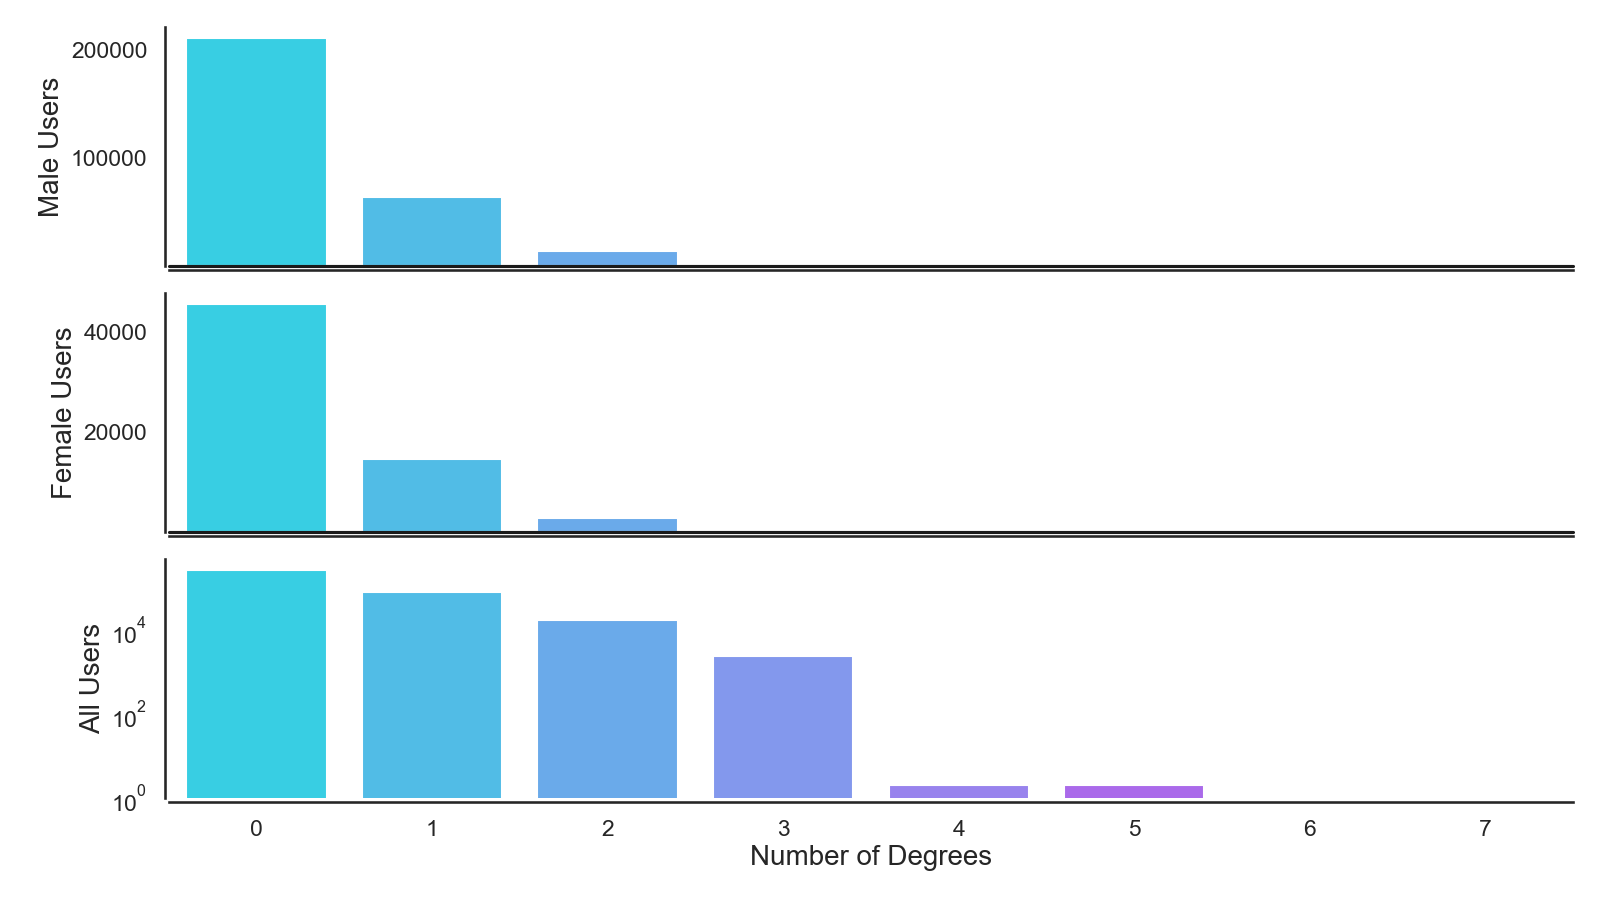
\includegraphics[width=\textwidth]{images/histogram/degrees_histogram.png}
        \caption{Istogramma dei titoli di studio}
        \label{fig:degreesbarplot}
    \end{subfigure}
\end{figure}
\begin{figure}[tb]\ContinuedFloat
    \begin{subfigure}{\textwidth}
        \centering
        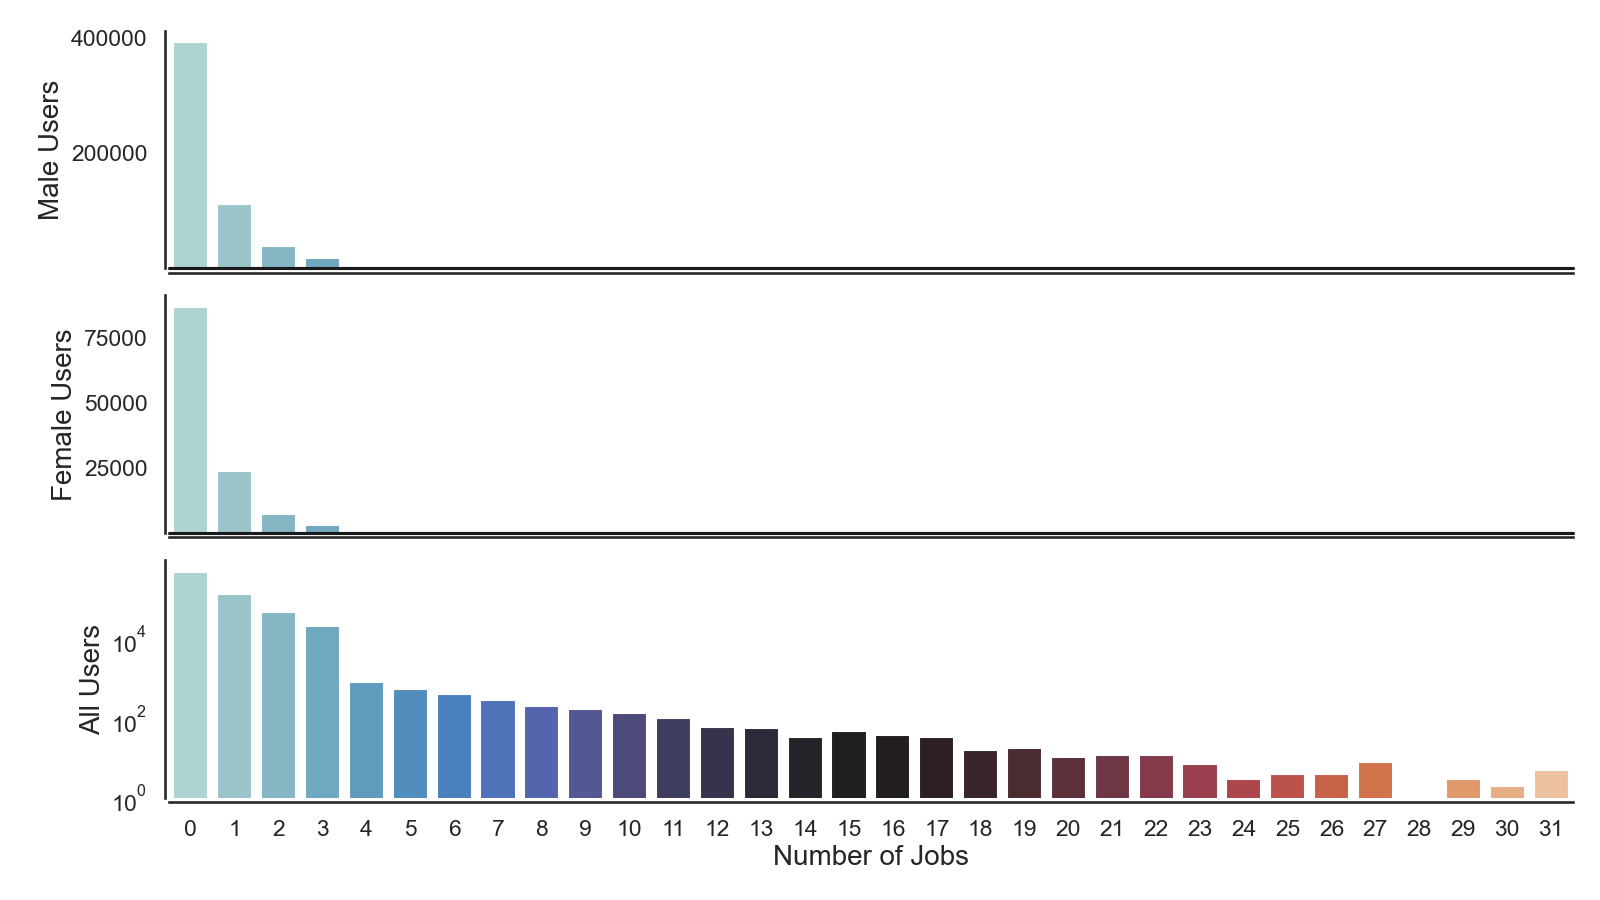
\includegraphics[width=\textwidth]{images/histogram/jobs_histogram.png}
        \caption{Istogramma dei lavori}
        \label{fig:jobsbarplot}
    \end{subfigure}
\end{figure}
La fase di \textit{preprocessig} ed estrazione delle scorte e dei flussi dai dati Crunchbase, ha avuto fondamento grazie un'analisi degli utenti Crunchbase. Questa ha determinato quale fosse la distribuzione dei titoli di studio e dei lavori sulla piattaforma. 
Il grafico in Figura \ref{fig:degreesbarplot} mostra che la maggior parte degli utenti ha tra uno e tre titoli di studio. 
Dalla Figura \ref{fig:jobsbarplot} si nota che maggior parte degli utenti ha avuto/ha almeno un lavoro.

Abbiamo definito la ``nazionalità'' come il paese più ricorrente tra le posizioni delle istituzioni presso le quali la persona ha ottenuto titoli di studio\footnote{A parità di numeri viene considerato il titolo di studio conseguito meno di recente.}. Se la nazionalità non è deducibile dai titoli di studio, ad esempio per mancanza della localizzazione delle istituzioni, si utilizza la posizione dell'azienda per cui l'utente ha lavorato meno di recente. 
La ''residenza'' è stata invece dedotta dai trasferimenti lavorativi degli utenti, definendola attraverso la posizione dell'azienda con la quale l'utente ha terminato il rapporto lavorativo.
\FloatBarrier
\begin{listing}[htbp]
\begin{minted}{Python}
def extractStocks(total=None, save=False, counter=0):
    my_db = NestedDict()
    if total is None:               |\label{caricatotalfile}| 
        total = read_total()
    if counter == 0:
        counter = count_jobs(total)
    with alive_bar(counter, title="Stocks", 
                   force_tty=True, spinner="classic") as stocks_bar:

        for person in total:        |\label{person_for_loop}| 
            ed_country := get_nationality(total[person]['degrees'], 
                                          total[person]['jobs'])
            if not len(total[person]['jobs']) or 
               not ed_country): |\label{checkifhavejobsgetNat}|
                continue
                
            for person_job in total[person]['jobs']:  |\label{person_jobs_for_loop}| 
                stocks_bar()
                if math.isnan(float(person_job['job_location'])) or 
                   math.isnan(float(person_job['job_start_date'])):     |\label{check_job_loc_date}|
                    continue
                    
                job_loc = person_job['job_location']
                job_start = dt.strptime(person_job['job_start_date'], 
                                            "%Y-%m-%d")
                if math.isnan(float(person_job['job_end_date'])):
                    if person_job['job_is_current']:
                        job_end = dt.strptime(2023, "%Y")
                    else:
                        continue
                else:
                    job_end = dt.strptime(person_job['job_end_date'],   |\label{check_job_loc_date_end}|
                                                      "%Y/%m/%d")
                                                      
                for year in range(2010, 2021):
                    year_t = dt.strptime(str(year), "%Y")
                    if year_t < job_start or year_t > job_end:
                        continue
    
                    gender = genderPrs(total[person]['person_gender'])   
                    my_db[ed_country][job_loc][str(year)][gender] += 1 |\label{stockSumLine}|
                |\label{person_jobs_for_loop_end}| 
        |\label{person_for_loop_end}| 
    if save:
        fileName = "Crunchbase Query Results/query_stocks_results.json"
        stockFile = open(fileName, "w+")
        stockFile.write(json.dumps(my_db, indent=4))
    return my_db
\end{minted}
\caption{Codice per l'estrazione delle scorte}
\label{lst:stockget}
\end{listing}

La Funzione \texttt{extractStocks(total=None, save=False, counter=0)} nel Codice \ref{lst:stockget} scorre i profili utente che possono essere passati in forma di dizionario oppure vengono caricati dalla memoria se presenti (riga \ref{caricatotalfile})). 
Per ogni utente si controlla che abbia avuto un impiego lavorativo e si estrapola la nazionalità dai titoli di studio (riga \ref{checkifhavejobsgetNat}). Successivamente si scorre la lista dei suoi lavori (righe \ref{person_jobs_for_loop} - \ref{person_jobs_for_loop_end}), e in questo ciclo si ottengono la posizione dell'azienda in cui ha lavorato e le date relative al rapporto lavorativo (righe \ref{check_job_loc_date} - \ref{check_job_loc_date_end}). Infine, si incrementano i valori delle scorte (in locale) in base ai dati che vengono incontrati (riga \ref{stockSumLine}). Come la Funzione \texttt{totalCreate()} nel Codice \ref{lst:tot_create}, anche questa permette di usare il parametro \texttt{save} per salvare il risultato; in ogni caso restituisce al chiamante le scorte calcolate.

Il preprocessig dei flussi viene effettuato mediante un processo identico a quello della Funzione \texttt{extactStocks()} nel Codice \ref{lst:stockget}, con un ciclo in più all'interno del ciclo dei lavori (righe \ref{person_jobs_for_loop} - \ref{person_jobs_for_loop_end}) per scorrere gli altri lavori dell'utente e confrontarne il periodo d'inizio e fine. Questo permette di stabilire se durante un determinato anno l'utente ha cambiato residenza.

\begin{listing}[htbp]
\begin{minted}{json}
{
    "USA": {    |\label{natState1}|
        "USA": {        |\label{destState1}|
            "2010": {   |\label{year1}|
                "male": 22,
                "female": 511082,
                "unknown": 1
            },          |\label{year1_end}|
        },
        "ITA": {        |\label{destState2}|
            "2015": {   |\label{year2}|
                "male": 0,
                "female": 11,
                "unknown": 0
            },
            "2016": {...}   |\label{year2_end}|
        },
    },
    "CAN": {...} |\label{natState2}|
}
\end{minted}
\caption{Codice di esempio scorte Academic Research Access}
\label{lst:stocksARA}
\end{listing}

Il metodo proposto ha premesso di ottenere le scorte di migranti organizzate nella medesima struttura di quelle nel MIMI dataset. Un esempio è mostrato nel Codice \ref{lst:stocksARA}. Il primo stato (e.g. righe \ref{natState1}, \ref{natState2}) indica la nazionalità delle scorte, il secondo (e.g. righe \ref{destState1}, \ref{destState2}) indica il paese in cui sono state conteggiate. Per ogni coppia si ha poi la lista degli anni con i relativi valori suddivisi per genere (righe \ref{year1}-\ref{year1_end}, \ref{year2}-\ref{year2_end}). 



\begin{listing}[htbp]
\begin{minted}{Python}
def common_items(d1, d2):
    return {k: common_items(d1[k], d2[k]) 
    if (k not in ["2010", "2015", "2020"]) and isinstance(d1[k], dict) |\label{istanceofdict}|
    else {'Crunchbase': sum(d1[k][e] for e in d1[k]), 
          'UN': int(d2[k]['total'])}
        for k in (d1.keys() & d2.keys())}   |\label{forallkey}| 
\end{minted}
\caption{Codice che interseca due dict}
\label{lst:dictIntersect}
\begin{minted}{Python}
def stocksIntersection(natStateFilter=None, stockStateFilter=None,
                       natContinentFilter=None, stockContinentFilter=None):
    cont = {}
    if natContinentFilter or stockContinentFilter:
        cont = dataextractor.read_json("Countries/ENA.json")
    stocks_query_file = "CrunchQR\stocks_results_with_jobs.json"
    un_stocks_file = "MIMI\Stocks\\UN_stocks.json"

    UN = dataextractor.read_json(un_stocks_file)                |\label{unstocksData}|
    crunchbase = dataextractor.read_json(stocks_query_file)     |\label{cbstockData}|
    result = common_items(crunchbase, UN)   |\label{dictintersections}|

    my_db = []
    for entry in result:            |\label{stockIntersectFor}|
        if (natContinentFilter and entry not in cont[natContinentFilter]) or \
                natStateFilter and entry != natStateFilter:
            continue
        for dest in result[entry]:
            if (stockContinentFilter and dest not in cont[stockContinentFilter]) or \
                    stockStateFilter and dest != stockStateFilter:
                continue
            for year in result[entry][dest]:
                my_db.append({'Origin': entry, 'Destination': dest, 'Year': year,
                              'Crunchbase': result[entry][dest][year]['Crunchbase'],
                              'UN': result[entry][dest][year]['UN']})
    |\label{stockIntersectFor_end}|

    df = pd.DataFrame(my_db)        |\label{dictToDataframe}|
    return df                       |\label{dictRetStocksIntersect}|
\end{minted}
\caption{Codice che interseca le scorte ufficiali con quelle Crunchbase}
\label{lst:stockIntersect}
\end{listing}


La Funzione ricorsiva \texttt{common\_items(d1, d2)} nel Codice \ref{lst:dictIntersect} effettua l'intersezione di due dict passati come parametro. Per ogni chiave k presente in entrambi i dizionari (\ref{forallkey}), se la chiave è istanza di dict viene richiamata ricorsivamente la funzione sui valori contenuto nei dizionari alla chiave k; altrimenti se la chiave è un numero compreso tra 2010, 2015 e 2020 (gli anni delle scorte in UN) viene ritornato il valore delle scorte presente in entrambi i dizionari. 
La Funzione \texttt{stockIntersection()} nel Codice \ref{lst:stockIntersect} carica i dati delle scorte (UN e Crunchbase) in locale (righe \ref{unstocksData}, \ref{cbstockData}). Se chiamata senza parametri restituisce il risultato della funzione \texttt{common\_items(d1, d2)} in un dataframe (righe \ref{dictintersections}, \ref{dictToDataframe}, \ref{dictRetStocksIntersect}). La Funzione \texttt{stockIntersection()} accetta quattro parametri come filtri: nazionalità, stato scorte, continente della nazionalità,  e continente delle scorte. Tutti i filtri vengono controllati all'interno del ciclo che scorre i dati ottenuti dall'intersezione di UN e Crunchbase (righe \ref{stockIntersectFor} - \ref{stockIntersectFor_end}). 


Il preprocessing descritto in questa sezione ha permesso di selezionare tutte le coppie di paesi (nazionalità - paese scorte) per cui sono presenti i dati sia nei dati ufficiali che in quelli Crunchbase. Ciò ha permesso di utilizzare i dati per la validazione delle scorte direttamente dalla struttura generata dalla Funzione \texttt{stockIntersection()} nel Codice \ref{lst:stockIntersect}. 

Per ottenere l'intersezione dei flussi Crunchbase con i flussi dei dati ufficiali è stato utilizzato un codice simile a quello per le scorte con un ciclo \texttt{for} ulteriore per scorre le residente degli utenti. Dato che per i flussi è stata usata la medesima struttura delle scorte, generata in fase di \textit{preprocessing} (Sezione \ref{preprocessing}). Con una leggera modifica che annida un ulteriore paese nel Codice Json \ref{lst:stocksARA} formando così una tripla cittadinanza-residenza-destinazione.

\section{Validazione dei flussi e scorte}
\label{analisidatiARA}
In questa sezione viene descritto il processo di validazione delle scorte e dei flussi collezionati da Crunchbase. 
Per visualizzare i dati migratori sono generati grafici di dispersione nei quali l'asse delle X rappresenta i dati di Crunchbase ottenuti mediante Academic Reseach Access e l'asse delle Y dai dati di confronto che possono essere dati Eurostat, UN o anche l'unione dei due. Ogni grafico presenta nella parte inferiore destra i valori delle correlazioni per validare i dati Crunchbase.  


\begin{listing}[htbp]
\begin{minted}{Python}
    df_matplot # ->> DATI INTERSECATI   |\label{intFunc}|
                    
    # GENERO TESTO CON TUTTE LE CORRELAZIONI
    string_on_plot = correlation_calc(df_matplot)  |\label{corrFunc}|

    # SCATTERPLOT
    p = sns.scatterplot()
    if stock: sns.regplot(x='Crunchbase',           |\label{trendLine}| 
                          y='Official', 
                          data=df_matplot)        
    plt.scatter(data=df_matplot,            |\label{scatterLine}| 
                x="Crunchbase", y="Official",        
                c="Crunchbase", cmap=color_map,
                edgecolors="black", linewidths=1, 
                alpha=0.6, s=100)                               |\label{scatterLine_end}|
    # RIGHT BAR
    cbar = plt.colorbar()
    
    # CORRELATIONS TEXT BOX                                 |\label{CorrAdd}|
    ob = offsetbox.AnchoredText(string_on_plot, loc="lower right", 
                                borderpad=2.5, prop=dict(size=15))
    ob.patch.set(boxstyle='round, pad=0.6')
    p.add_artist(ob)                                    |\label{CorrAdd_end}|
\end{minted}
\caption{Codice per realizzare i grafici di dispersione}
\label{lst:getScatter}
\end{listing}

Il Codice \ref{lst:getScatter} genera un grafico a dispersione con i valori Crunchbase sull'asse orizzontale e i valori dei dati ufficiali sull'asse verticale (righe \ref{scatterLine} - \ref{scatterLine_end}). Inoltre, solo per le scorte, genera una linea che indica la tendenza che hanno i valori delle scorte (riga \ref{trendLine}). Infine, aggiunge il riquadro delle correlazioni al grafico (righe \ref{CorrAdd} - \ref{CorrAdd_end}). La correlazione viene calcolata dalla Funzione \texttt{correlation\_calc()} (Codice \ref{lst:corrCalc}).


\begin{listing}[htbp]
\begin{minted}{Python}
def correlation_calc(df, source_="UN", flows=None):
    crunch = "Crunchbase"                                       |\label{confrCB}|
    source = source_                                            |\label{confrSource}|
    out = {}
    PearsLogOf = "PearsonLog" + source
    el = "_cit" if flows else ""                                |\label{citresFlows}|
    while True:                                                 |\label{whileFlows}|
        if df[crunch + el].any() and df[source + el].any():
            np.seterr(divide='ignore')
            
            # MASK INVALID VALUES
            maCruch = np.ma.masked_invalid(df[crunch + el])   |\label{crMask}|
            maOff = np.ma.masked_invalid(df[source + el])     |\label{ofMask}|
            logMaCruch = np.log(maCruch)   
            logMaOff = np.log(maOff)    
            
            # PEARSON CORR CALC                                 |\label{corrca}|
            out["Pearson" + el] = round(
                np.ma.corrcoef(maCruch, maOffDF)[0][1], 2)
            out["PearsonLog" + el] = round(
                np.ma.corrcoef(logMaCrunch, logMaOff)[0][1], 2)
            out[PearsLogOf + el] = round(
                np.ma.corrcoef(maCruch, logMaOff)[0][1], 2)
            out["PearsonLogCB" + el] = round(
                np.ma.corrcoef(logmaCrunch, maOffDF)[0][1], 2)

            # SPEARMAN CORR CALC
            df_corr_spearman = df.corr(method='spearman')
            out["Spearman" + el] = round(
                df_corr_spearman[crunch + el][source + el], 2)  |\label{corrca_end}|

            if flows:
                if el == "_cit":
                    el = "_res"
                    continue
            break

    # TO STRING
    if flows:
    new_d = "\n".join("{}: {!r}".format(k, out[k])
                      for k in sorted(out, key=len, reverse=False) 
                      if k.endswith("_cit"))
    new_d2 = "\n".join("{}: {!r}".format(k, out[k])
                       for k in sorted(out, key=len, reverse=False) 
                       if k.endswith("_res"))
    return new_d, new_d2

    return "\n".join("{}: {!r}".format(k, out[k])
                     for k in sorted(out, key=len, reverse=False))
\end{minted}
\caption{Codice per il calcolo delle correlazioni}
\label{lst:corrCalc}
\end{listing}
La Funzione \texttt{correlation\_calc()} nel Codice \ref{lst:corrCalc} genera una stringa contenente le correlazioni di Pearson e Spearman per i dati all'interno del dataframe, parametro della funzione. La funzione è strutturata per adattarsi al calcolo di correlazioni sia per stock che per flussi. Infatti, attraverso il parametro flows è possibile dire se il dataset passato si riferisce a flussi migratori (di default si calcolano le scorte).
Il Codice, per le scorte, si aspetta di trovare nel dataframe passato colonne con i nomi ''Crunchbase'' (riga \ref{confrCB}) e la stringa passata nel parametro source\_(riga \ref{confrSource}). 
Vengono mascherati i dati invalidi in entrambi i dataset con valori pari a 0 (righe \ref{crMask}, \ref{ofMask}), e successivamente vengono calcolare le varie correlazioni (righe \ref{corrca} - \ref{corrca_end}). Se il parametro flows è True, le colonne cercate nel dataframe saranno composte dal nome delle fonti (Crunchbase o fonte ufficiale) e da ''\_cit'' o ''\_res'' (riga \ref{citresFlows}), ed inoltre tutti i calcoli verranno eseguiti sia per i cittadini che per i residenti (riga \ref{whileFlows}).

La correlazione di Pearson ci dice se vi è una relazione lineare tra due variabili. Anche se il coefficiente di correlazione di Pearson indica che non ci sia correlazione lineare potrebbe esistere una relazione di altro tipo. Per questo motivo, i dati vengono sottoposti anche al calcolo del coefficiente di correlazione per ranghi di Spearman, che determina relazioni monotone. Quando i due indici sono vicini abbiamo una conferma della relazione


\section{Metodi e strumenti utilizzati}
\label{strumentiutilizzati}
Tutto il codice è stato scritto in Python e sviluppato utilizzando l'IDE PyCharm. E' stata utilizzata la versione \textit{education} fornita agli studenti dall'Università di Pisa, che ha svolto le operazioni di installazione delle librerie in modo automatico. 
Le librerie Python utilizzate riguardano:
\begin{itemize}
\item lettura di file JSON: json; 
\item manipolazione dei dati: dict, pandas\footnote{\url{https://pandas.pydata.org/docs/}}, alive-progress \cite{rsalmei} usata per determinare lo stato del processo;;
\item realizzazione di grafici: matplolib \cite{Hunter:2007}, seaborn \cite{Waskom2021}. Inoltre, plotapi\footnote{Plotapi: \url{https://plotapi.com/}} è stata usata per visualizzare in grafici circolari le scorte ed i flussi; 
\item calcolo delle correlazioni: NumPy \cite{harris2020array} per Pearson, e pandas per Spearman
\end{itemize}

%% Non è necessaria, momentaneamente
%\begin{comment}
\subsection{Correlazione}
L'Indice di correlazione è una misura che ci permette di stabilire quanto due insiemi di dati siano correlati, ovvero quanto i valori di uno dipendono dall'altro. 
I due indici di interesse per questo elaborato sono l'indice di Pearson per correlazioni lineari \cite{pearson} e l'indice di Spearman per correlazioni non lineari \cite{10.2307/2284441}. In questo elaborato abbiamo utilizzato l'indice di correlazione per validare i flussi e scorte migratorie estratte da Crunchbase.

\paragraph{Pearson}
Pearson impone alcune condizioni per i dati:
\begin{itemize}
\item Le due variabili devono essere entrambe di tipo quantitativo;
\item Le due variabili devono avere dati che si riferiscono allo stesso caso;
\item Le due variabili a confronto devono avere una crescita lineare, se questo non avviene si trasformano una o entrambe le variabili secondo una scala logaritmica;
\item Non devono esserci Outliers tra i dati\footnote{Un dato che si discosta di molto rispetto agli altri};
\item Entrambe le variabili devono avere una distribuzione normale, che può essere verificata per campioni minori ai 5000 valori tramite il test di Shapiro-Wilk\footnote{Test per verificare la normalità}.
\end{itemize}
Il coefficiente di correlazione di Pearson per due variabili random si calcola partendo dalla covarianza delle variabili  :
\[\rho(X,Y)  = \frac{COV(XY)}{\sigma(X) \sigma(Y)}\]
Dove \(COV(XY)\) indica la covarianza tra le due variabili e \(\sigma(X)\) e \(\sigma(Y)\) indicano la deviazione standard rispettivamente per X e per Y.


\paragraph{Spearman}
 I criteri che permettono di sfruttare questo coefficiente si fermano ai primi due step dell'indice di Pearson, il coefficiente di Spearman si può infatti definire come un caso specifico di indice di Pearson in cui si trasformano i dati in ranghi prima di calcolare il coefficiente. 
\[\rho _{s}={\frac {\sum _{i}(r_{i}-{\overline {r}})(s_{i}-{\overline {s}})}{{\sqrt {\sum _{i}(r_{i}-{\overline {r}})^{2}}}{\sqrt {\sum _{i}(s_{i}-{\overline {s}})^{2}}}}}\]
In applicazioni pratiche si utilizza una formula semplificata: \(\rho _{s}=1-{\frac {6\sum _{i}D_{i}^{2}}{N(N^{2}-1)}}\) dove \(D_i\) rappresenta la differenza tra i ranghi \(r_{i}-s_{i}\) delle due variabili confrontate. \\

Interpretazione degli indici:
\begin{itemize}
    \item Se l'indice \(\rho > 0\) si definiscono X e Y come variabili correlate positivamente.
    \item Se l'indice \(\rho = 0\) non c'è correlazione tra le due variabili.
    \item Se l'indice \(\rho < 0\) si definiscono X e Y come variabili correlate negativamente.
\end{itemize}


%In base al caso specifico, se c'è correlazione sia che sia positiva o negativa questa viene suddivisa in più gruppi ovvero:
%\begin{itemize}
%    \item Se \(0 <= |\rho| <= 0,3 \) si ha correlazione debole 
%    \item Se \(0,3 < |\rho| <= 0,7 \) si ha correlazione moderata 
%    \item Se \(0,7 < |\rho| <= 1 \) si ha correlazione forte 
%\end{itemize}
%\end{comment}

\section{Conclusione}
In questo capitolo è stato descritto l'approccio utilizzato per accedere, collezionare e analizzare i dati. 
L'analisi del funzionamento della piattaforma Crunchbase (Sezione \ref{sottosezionequerybuilder}), ha permesso di sviluppare un algoritmo di collezione dei dati (Sezione \ref{customquerybuilder}). 
Mediante l'accesso diretto ai dati di Crunchbase (Sezione \ref{academic_access_section}) è stato reso più rapido il calcolo delle scorte e dei flussi. 

Da un analisi dei dati si determina che buona parte degli utenti ha almeno 1 titolo di studio ed ha avuto più di due lavori. Queste proprietà sono fondamentali affinché attraverso l'assunzione fatta per stabilirne la nazionalità si possa procedere con l'analisi ed il confronto con dati veri.
L'analisi dei dati, ottenuti attraverso l'Academic Research Access, è stata svolta mediante librerie Python (Sezione \ref{strumentiutilizzati}) che hanno permesso di manipolare i dati (Sezioni \ref{preprocessing}), realizzare i grafici e calcolare le varie correlazioni (Sezioni \ref{analisidatiARA}).